
\section{\nmu Algoritmos de \textit{string matching} exatos} % (fold)
\label{sec:algor_timos_de_string_matching_exatos}

Para a busca com algoritmos de \textit{string matching} exatos, foram considerado três abordagens distintas:

\begin{description}
	\item[Expressão Regular:] Método atual de verificação. Foi comentado previamente  na \autoref{sec:algoritimos_de_textit}.
	\item[Knuth-Morris-Pratt:] Algoritmo que faz de uso do conceito de autômatos de estados para acelerar a busca. Previamente apresentado na \autoref{ssub:knuth_morris_pratt_}.
	\item[Rabin-Karp:]  Algoritmo que faz de uso de \textit{hash}. Ver \autoref{ssub:rabin_karp}.
\end{description}

Após a coleta de $150$ execuções de busca para dez pacotes usando os algoritmos apontados acima, a \autoref{ssub:rabin_karp} foi elaborada a partir da a mediana dos tempos destas execuções.

\begin{figure}[htbp]
  \centering
  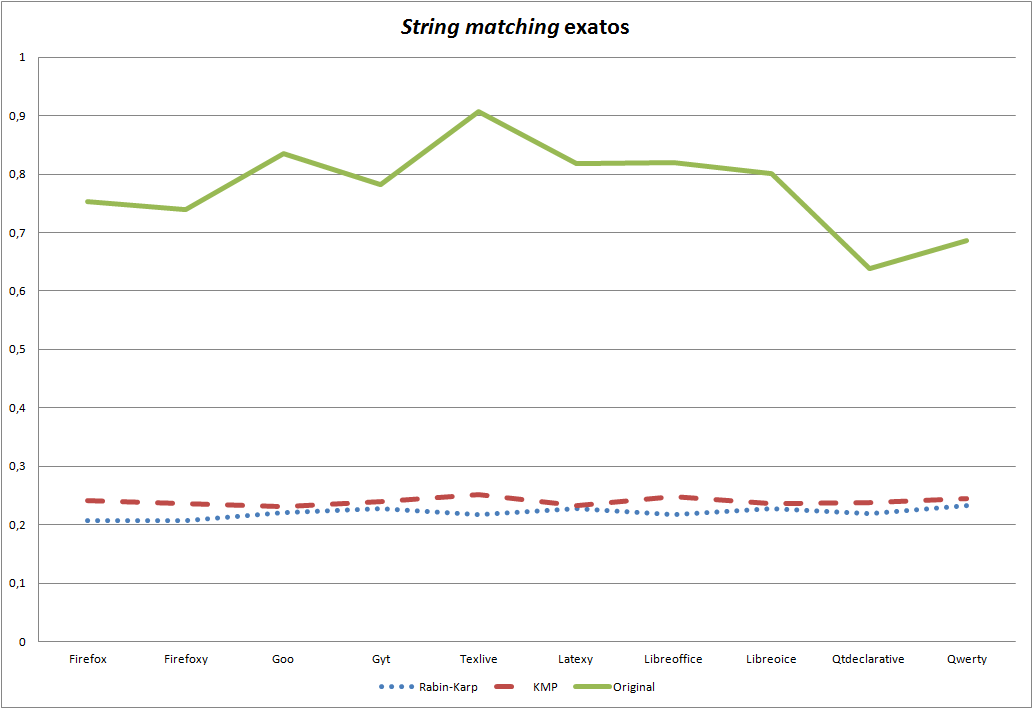
\includegraphics[width=0.95\textwidth]{figuras/tempo-rk_kmp_std}
  \caption{Estimativa de tempo para pacotes usando algoritmos de busca exata}
  \label{tempo_rk_kmp_std}
\end{figure}

Como podemos observar, tanto o \textit{Rabin-Karp} quanto o \textit{KMP} tiveram um tempo de execução de cerca de $\frac{1}{3}$ do tempo gasto atualmente com o uso de expressões regulares, sendo que, no geral, o algoritmo de \textit{Rabin-Karp} possui um desempenho ligeiramente melhor.


\begin{figure}[htbp]
  \centering
  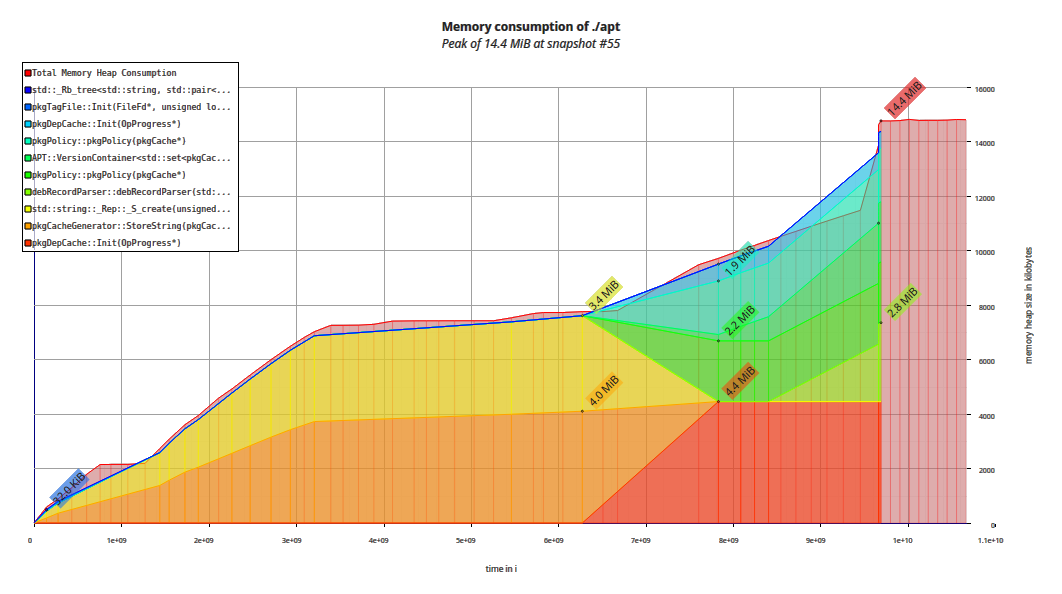
\includegraphics[width=0.95\textwidth]{figuras/memory_rk.png}
  \caption{Uso de memória com uso do algoritmo de \textit{Rabin-Karp}}
  \label{memory_rk}
\end{figure}

O consumo total de memória para ambos os algoritmos, \textit{Rabin-Karp} na \autoref{memory_rk} e expressões regulares na \autoref{memory_std},  apresentaram resultados similares, porém o método de \textit{Rabin-Karp} faz um uso de memória mais pontual, alcançando o pico de consumo ao final do processo, quando esta prestes a liberar os recursos. Já o método de expressões regulares apresenta um consumo aproximadamente linear de memória. 


\begin{figure}[htbp]
  \centering
  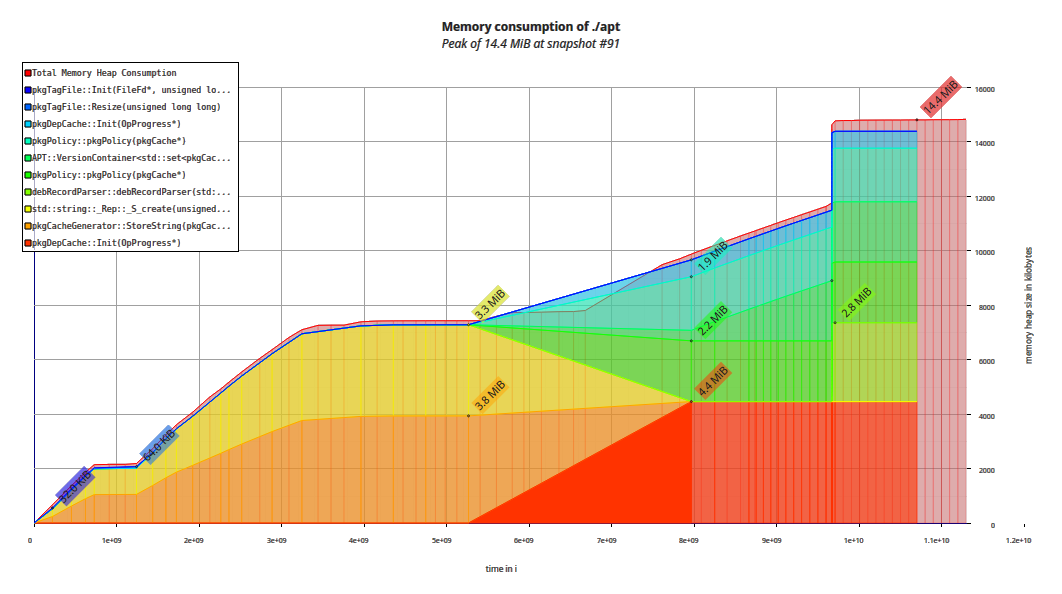
\includegraphics[width=0.95\textwidth]{figuras/memory_regex.png}
  \caption{Uso de memória das expressões regulares}
  \label{memory_std}
\end{figure}

Um gasto mais prologado de memória vem a ser prejudicial para sistemas em que diversos processos possam estar sendo executados em conjunto; Todavia, o grau de consumo é baixo, evitando que este consumo por um período mais extenso venha a ser prejudicial. Em um sistema com 2GB de memória RAM, os 15MB utilizados representam menos de $1\%$ do total dos recursos disponíveis.
% chapter analise_de_resultados (end)

